% =============================================================================
% MiniReplication.tex — first end-to-end practice deck
%
% Synthetic panel -> Stata (reghdfe/esttab) -> Matplotlib -> Beamer.
% No real data; every number and figure is produced by scripts (Art. I).
%
% Compile (3 passes, no bibliography):
%   cd Slides && TEXINPUTS=../Preambles:$TEXINPUTS xelatex MiniReplication.tex
% =============================================================================

\documentclass{beamer}
\usepackage{xeCJK}
\xeCJKsetup{PunctStyle=kaiming}
\setCJKmainfont{PingFang SC}
\setCJKsansfont{PingFang SC}
\input{header}

\title{全链路迷你复现:干旱、水电与工业产出}
\subtitle{合成数据 · Stata · Matplotlib · Beamer}
\author{Workflow Practice Sandbox}
\date{2026-10-28 \quad \muted{练习沙盒 · 合成数据}}

\begin{document}

\frame{\titlepage}

\begin{frame}{动机}
  \begin{itemize}
    \item 沙盒的\key{第一个全链路练习}:一次跑通 Stata、Python 与 \LaTeX
    \item 主题仿照真实研究:干旱减少水电,水电影响工业产出
    \item 数据\muted{全部合成},真值已知,可检验估计量是否回到真值
    \item 每个数字、每张表、每张图都由脚本生成,讲稿只负责引用
  \end{itemize}
\end{frame}

\begin{frame}{数据生成过程}
  \begin{itemize}
    \item 干旱指数 $D_{it}$ 为 AR(1)($\rho = 0.6$),标准化后标准差为 1
    \item 降水异常 $P_{it} = -0.5\,D_{it} + \omega_{it}$,同样标准化
    \item 水电份额 $H_{it} = \alpha_i - 0.04\,D_{it} + v_{it}$
    \item 工业产出 $\ln Y_{it} = \eta_i + \lambda_t + 2.0\,H_{it} - 0.010\,P_{it} + \varepsilon_{it}$
  \end{itemize}
  \vspace{0.3em}
  \begin{itemize}
    \item 真值:$\beta = 0.04$,$\theta = 2.0$,$\gamma = -0.010$
    \item 样本:31 省 $\times$ 20 年(2000--2019),$N = 620$
    \item 随机项:$v \sim N(0, 0.03^2)$,$\varepsilon \sim N(0, 0.12^2)$
  \end{itemize}
\end{frame}

\begin{frame}{变量关系}
  % Diagram: synthetic DGP -- drought drives the hydro share and the
  % precipitation anomaly; both shape industrial output.
  % Coordinates: D(0,0) H(3.2,0) Y(6.4,0) P(3.2,2.0); nodes text width 1.6cm
  \centering
  \begin{tikzpicture}
    \node[dag-node, text width=1.6cm] (D) at (0,0) {$D_{it}$\\干旱};
    \node[dag-node, text width=1.6cm] (H) at (3.2,0) {$H_{it}$\\水电};
    \node[dag-node, text width=1.6cm] (Y) at (6.4,0) {$Y_{it}$\\产出};
    \node[dag-node, text width=1.6cm] (P) at (3.2,2.0) {$P_{it}$\\降水};
    \draw[observed-edge] (D) -- (H) node[midway, above] {$-\beta$};
    \draw[observed-edge] (H) -- (Y) node[midway, above] {$+\theta$};
    \draw[observed-edge] (P) -- (Y) node[midway, right] {$-\gamma$};
    \draw[observed-edge] (D) -- (P) node[midway, above left] {$-0.5$};
  \end{tikzpicture}

  \vspace{0.8em}
  \begin{itemize}
    \item 省与年的固定效应被吸收,不画入图
    \item $P$ 由 $D$ 生成,并直接进入产出方程
  \end{itemize}
\end{frame}

\begin{frame}{数据概览}
  \begin{center}
    {
\def\sym#1{\ifmmode^{#1}\else\(^{#1}\)\fi}
\begin{tabular}{l*{1}{cc}}
\toprule
                    &\multicolumn{2}{c}{}     \\
                    &        Mean&   Std. Dev.\\
\midrule
Hydro share (0-1)   &       0.317&       0.095\\
Drought index (std.)&      -0.000&       1.001\\
Precip. anomaly (std.)&      -0.000&       1.001\\
Log industrial output&      11.567&       0.426\\
\bottomrule
\end{tabular}
}

  \end{center}
  \begin{itemize}
    \item 31 省 $\times$ 20 年 = 620 个观测,无缺失
    \item $D$ 与 $P$ 已标准化(均值 0,标准差约 1)
    \item 水电份额均值约 0.32,范围 0.07--0.59
  \end{itemize}
\end{frame}

\begin{frame}{估计方法}
  \begin{itemize}
    \item 每个设定都带省与年双向固定效应:\texttt{reghdfe} 吸收双向 FE
    \item 标准误在省级聚类(31 个聚类)
    \item (1) 仅 $H$;(2) 加 $P$;(3) 仅 $D$(总关联);(4) 三者同时
    \item (5) 二次项 $D^2$ 的证伪检验,未进表
    \item 表与图由脚本生成,讲稿只引用生成物
  \end{itemize}
\end{frame}

\transitionslide{结果}

\begin{frame}{回归结果}
  \begin{center}
    \resizebox{\textwidth}{!}{{
\def\sym#1{\ifmmode^{#1}\else\(^{#1}\)\fi}
\begin{tabular}{l*{4}{c}}
\toprule
                    &\multicolumn{1}{c}{(1)}&\multicolumn{1}{c}{(2)}&\multicolumn{1}{c}{(3)}&\multicolumn{1}{c}{(4)}\\
                    &\multicolumn{1}{c}{Baseline}&\multicolumn{1}{c}{+ Precip.}&\multicolumn{1}{c}{Drought only}&\multicolumn{1}{c}{Direct effect}\\
\midrule
h                   &       1.961\sym{***}&       1.960\sym{***}&                     &       1.793\sym{***}\\
                    &      (0.11)         &      (0.11)         &                     &      (0.15)         \\
\addlinespace
p                   &                     &       0.000         &                     &      -0.003         \\
                    &                     &      (0.01)         &                     &      (0.01)         \\
\addlinespace
d                   &                     &                     &      -0.082\sym{***}&      -0.012         \\
                    &                     &                     &      (0.01)         &      (0.01)         \\
\midrule
Observations        &         620         &         620         &         620         &         620         \\
Adj. R-squared      &       0.922         &       0.922         &       0.907         &       0.922         \\
\bottomrule
\multicolumn{5}{l}{\footnotesize SEs in parentheses, clustered at province level (31 clusters).}\\
\multicolumn{5}{l}{\footnotesize * p<0.10, ** p<0.05, *** p<0.01.}\\
\end{tabular}
}
}
  \end{center}
  \begin{itemize}
    \item $H$ 的系数为 1.96 (0.11),与真值 $\theta = 2.0$ 相差不足 0.05
    \item 控制 $H$ 后,$D$ 的系数为 $-0.012$ (0.011),不再显著
  \end{itemize}
\end{frame}

\begin{frame}{图 1:水电份额与干旱指数}
  \begin{center}
    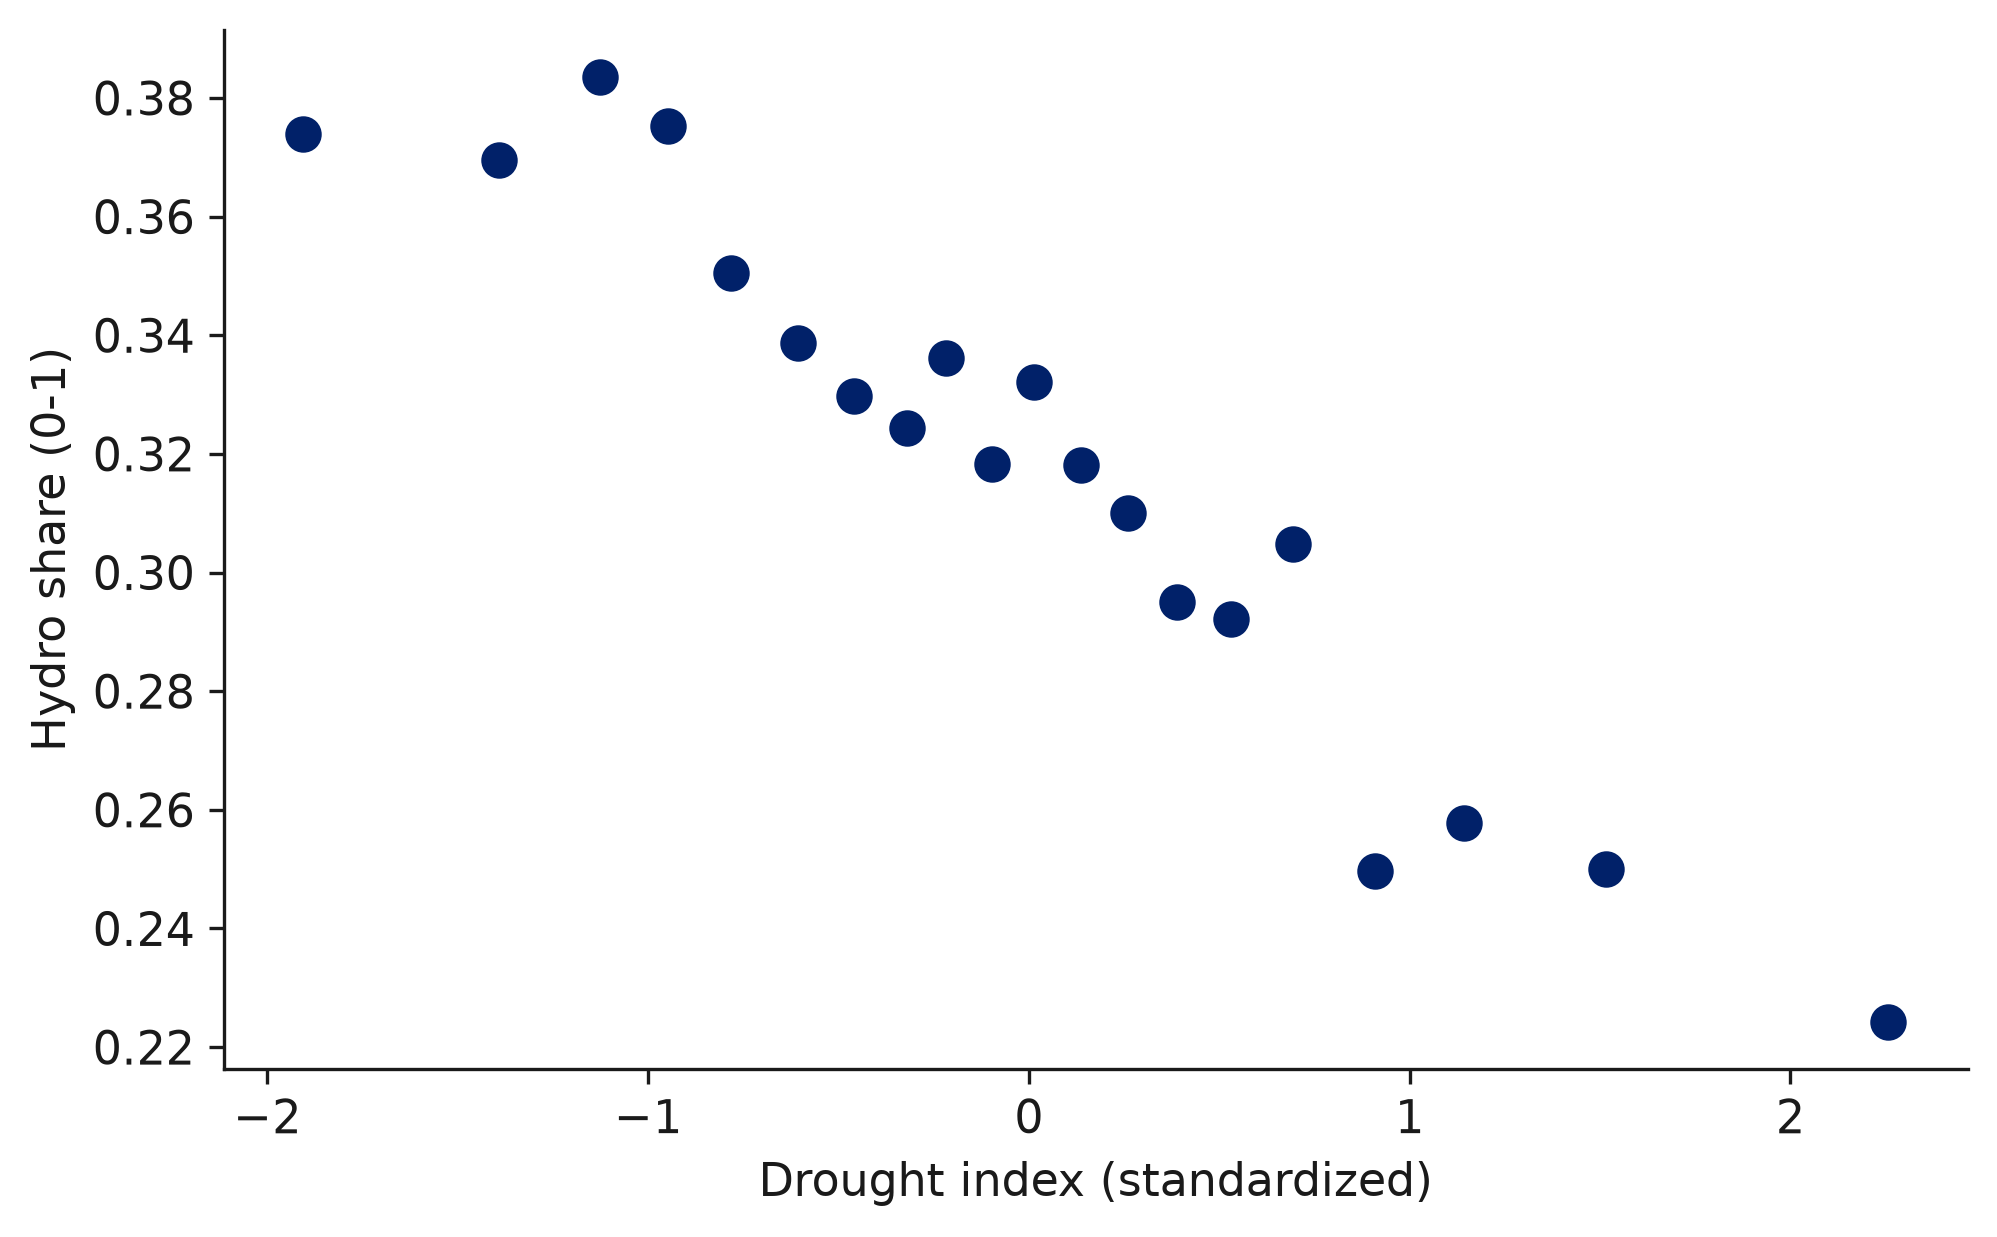
\includegraphics[width=0.78\textwidth]{../output/figures/fig_hydro_by_drought_bins.png}
  \end{center}
  \begin{itemize}
    \item 20 个等频分箱:干旱指数越高,水电份额越低
    \item 方向与量级与 DGP 的 $\beta = 0.04$ 一致
  \end{itemize}
\end{frame}

\begin{frame}{图 2:系数估计}
  \begin{center}
    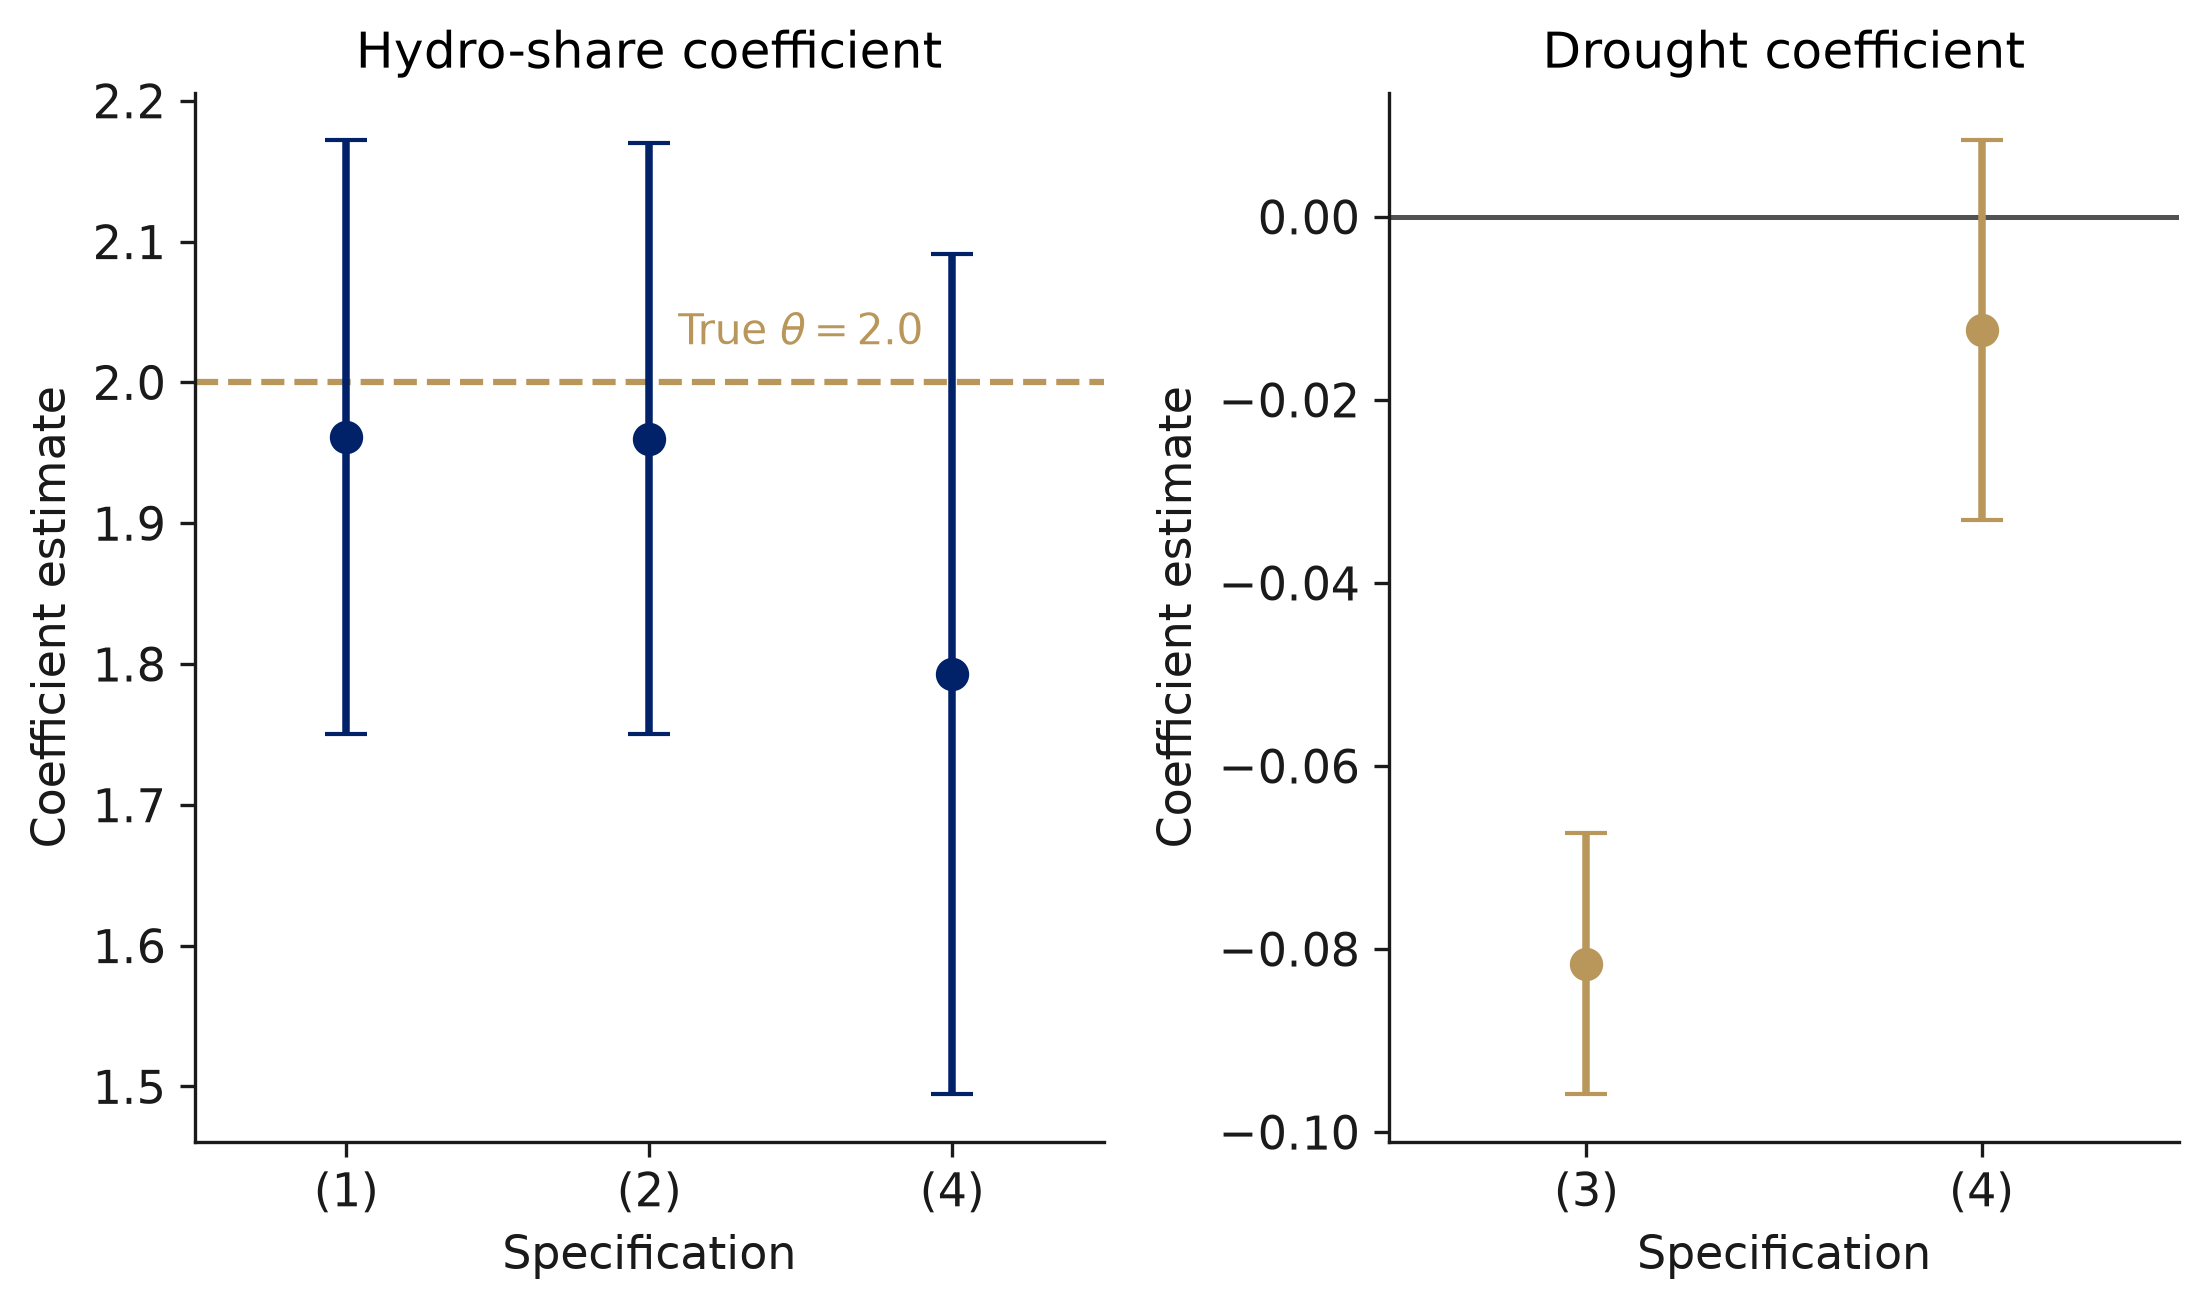
\includegraphics[width=0.80\textwidth]{../output/figures/fig_coefplot.png}
  \end{center}
  \begin{itemize}
    \item $H$ 的系数在 (1)、(2)、(4) 中均接近真值 2.0;(4) 的区间更宽
    \item $D$ 的总关联为 $-0.082$;控制 $H$ 后直接效应 $-0.012$,区间覆盖 0
  \end{itemize}
\end{frame}

\begin{frame}{要点}
  \begin{itemize}
    \item \good{管线跑通}:数据 $\to$ 估计 $\to$ 表 $\to$ 图 $\to$ 讲稿,一条命令复现
    \item \key{权威源}:表与图只由脚本生成,讲稿不手写数字
    \item \key{可复现}:种子置顶、相对路径、esttab 直出 \LaTeX
    \item \key{发表级}:矢量 PDF + 300 dpi 透明 PNG,项目调色板
    \item 学习点:估计量回到已知真值,证伪检验也通过
  \end{itemize}
\end{frame}

\begin{frame}{下一步}
  \begin{itemize}
    \item 换真实数据,重跑同一套编号管线
    \item 安装 Quarto 后,把本稿翻译成 RevealJS 版本
    \item 把 spec-ledger 的追加习惯用到每个新设定上
    \item 用 \texttt{/commit} 走完整质量门后提交本章产物
  \end{itemize}
\end{frame}

\end{document}
